\documentclass[11pt]{article}
\usepackage{graphicx}
\usepackage{hyperref}
\usepackage{amsmath}
\usepackage{listings}
\usepackage{color}
\usepackage{geometry}
\geometry{margin=1in}

\usepackage{tikz}
\usetikzlibrary{shapes.geometric, arrows.meta, positioning}

\tikzstyle{process} = [rectangle, minimum width=3.8cm, minimum height=1.2cm, text centered, draw=black, fill=blue!10]
\tikzstyle{decision} = [diamond, minimum width=3.8cm, minimum height=1cm, text centered, draw=black, fill=yellow!30, aspect=2]
\tikzstyle{terminator} = [rectangle, rounded corners, minimum width=3.8cm, minimum height=1.2cm, text centered, draw=black, fill=gray!15]
\tikzstyle{arrow} = [thick,->,>=stealth]

\title{CPER Environmental Product Declarations (EPD) Search Workflow}
% \author{Stirunag P. \\ \texttt{stirunag@example.com}}
\date{\today}

\definecolor{lightgray}{gray}{0.95}
\lstset{
  backgroundcolor=\color{lightgray},
  basicstyle=\ttfamily\footnotesize,
  frame=single,
  breaklines=true
}

\begin{document}

\maketitle

\begin{abstract}
This report outlines the complete end-to-end pipeline for processing, indexing, and querying Environmental Product Declarations (EPDs) based on the ``Global Warming Potential'' impact category. The solution involves preprocessing JSON data, constructing a searchable FAISS index using bi-encoder sentence embeddings, and refining query matches using a cross-encoder for semantic re-ranking. We use FastAPI to deploy the model as an interactive search interface.
\end{abstract}

\section{Introduction}
Environmental Product Declarations (EPDs) provide quantified environmental data for products under standardized conditions. In CPER, we focus on retrieving semantically similar EPDs given a user query to extract meaningful impact data such as A1–A5 lifecycle indicators.

The system uses both \textbf{bi-encoder} models for fast vector similarity and \textbf{cross-encoder} models for accurate re-ranking, creating a powerful hybrid search engine.

\begin{figure}[htbp]
    \centering

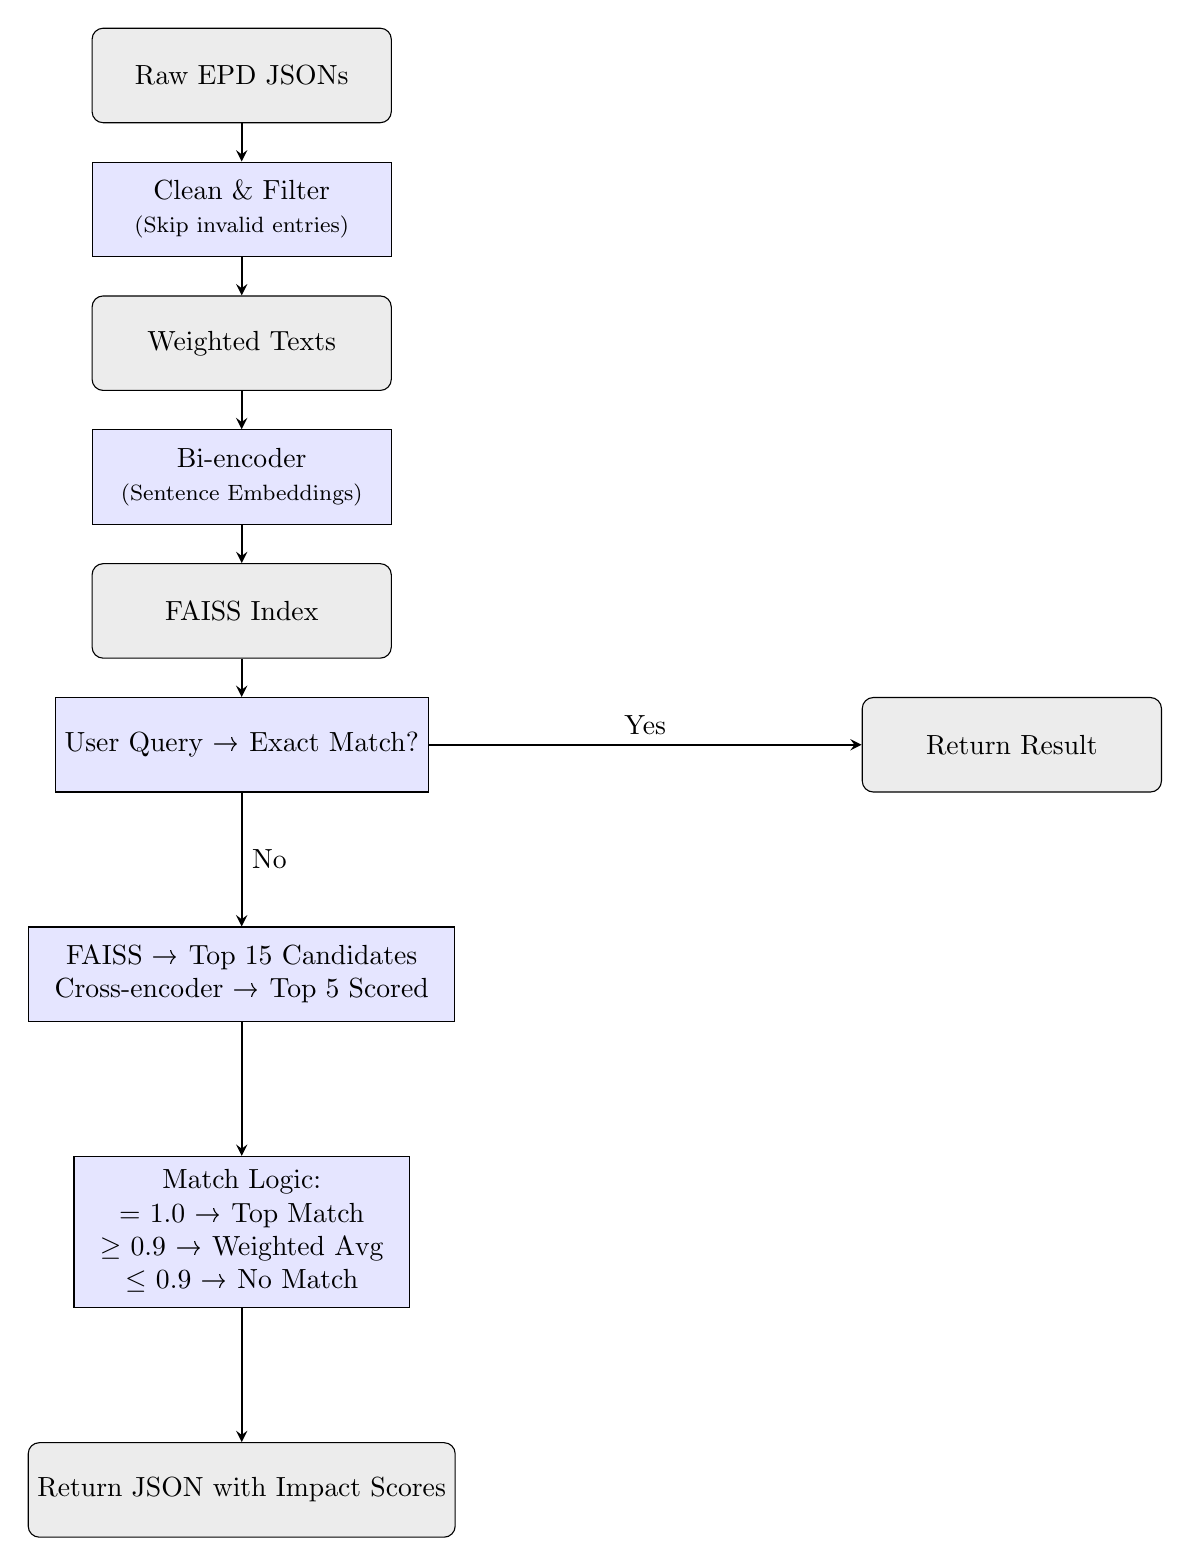
\begin{tikzpicture}[node distance=1.7cm]

% Main linear flow
\node (start) [terminator] {Raw EPD JSONs};
\node (clean) [process, below of=start] {
    \begin{tabular}{c}
    Clean \& Filter \\
    \footnotesize (Skip invalid entries)
    \end{tabular}
};

\node (text) [terminator, below of=clean] {Weighted Texts};
\node (embed) [process, below of=text] {
    \begin{tabular}{c}
    Bi-encoder \\
    \footnotesize (Sentence Embeddings)
    \end{tabular}
};
\node (faiss) [terminator, below of=embed] {FAISS Index};
\node (query) [process, below of=faiss] {User Query → Exact Match?};

% Branch: exact match
\node (match) [terminator, right=5.5cm of query] {Return Result};

% FAISS + cross-encoder branch
\node (faiss2) [process, below=1.7cm of query] {
    \begin{tabular}{c}
    FAISS → Top 15 Candidates \\
    Cross-encoder → Top 5 Scored
    \end{tabular}
};

\node (logic) [process, below=1.7cm of faiss2] {
    \begin{tabular}{c}
    Match Logic: \\
    $=$ 1.0 → Top Match \\
    $\geq$ 0.9 → Weighted Avg \\
    $\leq$ 0.9 → No Match
    \end{tabular}
};

\node (return) [terminator, below=1.7cm of logic] {Return JSON with Impact Scores};

% Arrows
\draw [arrow] (start) -- (clean);
\draw [arrow] (clean) -- (text);
\draw [arrow] (text) -- (embed);
\draw [arrow] (embed) -- (faiss);
\draw [arrow] (faiss) -- (query);
\draw [arrow] (query) -- node[above] {Yes} (match);
\draw [arrow] (query) -- node[right] {No} (faiss2);
\draw [arrow] (faiss2) -- (logic);
\draw [arrow] (logic) -- (return);

\end{tikzpicture}

    \caption{Workflow of the CPER EPD semantic search system. The user query is processed through exact match, FAISS-based filtering, and cross-encoder re-ranking to determine impact data.}
    \label{fig:epd-workflow}
\end{figure}

As shown in Figure~\ref{fig:epd-workflow}, the semantic search pipeline begins with cleaning and embedding...


\section{Data Processing}
Raw EPD data is provided as JSON files. We begin by parsing each file and applying strict validation to ensure quality. Each entry must meet the following criteria:

\begin{itemize}
    \item The \texttt{epd\_impacts} must include the ``Global Warming'' impact category.
    \item All relevant impact values (A1, A2, A3, A4, A5, A1\_A3\_total) must not all be zero or null.
    \item The \texttt{product\_names}, \texttt{product\_ids}, and \texttt{product\_description} must not be placeholders.
\end{itemize}

Valid entries are normalized and cleaned, and only the relevant impact category is preserved. The output is saved as \texttt{processed\_json\_data.json}.

\section{Text Representation}
To facilitate semantic search, each valid EPD is converted into a weighted text representation:

\begin{lstlisting}
combined_text = (product_name * 3) + (product_id * 2) + product_description
\end{lstlisting}

This boosts the importance of the name and ID in similarity calculations.

\section{Sentence Embedding and FAISS Indexing}
We use the \texttt{all-MiniLM-L6-v2} model from \texttt{sentence-transformers} to encode each EPD into a dense vector embedding. These embeddings are normalized and stored in a FAISS \texttt{IndexFlatIP}, enabling fast inner-product searches (which approximate cosine similarity).

The following files are generated:
\begin{itemize}
    \item \texttt{revised\_faiss\_index.index}: FAISS index
    \item \texttt{revised\_json\_mapping.pkl}: JSON mapping (EPDs)
    \item \texttt{embedding\_model\_name.txt}: Embedding model reference
\end{itemize}

\section{Hybrid Search Pipeline}
The user query flows through the following steps:

\begin{enumerate}
    \item \textbf{Exact Match Check}: Compares query directly with product names, IDs, and descriptions.
    \item \textbf{FAISS Search}: Embeds the query using the same bi-encoder and retrieves top-K candidate EPDs.
    \item \textbf{Cross-Encoder Re-ranking}: Each candidate is paired with the query and passed to a \texttt{cross-encoder/ms-marco-MiniLM-L-6-v2} model for a more accurate similarity score.
\end{enumerate}

\subsection*{Scoring Logic}
\begin{itemize}
    \item \textbf{Similarity = 1.0}: Return top match.
    \item \textbf{Similarity $\geq$ 0.9}: Compute weighted average from top matches.
    \item \textbf{Similarity $<$ 0.9}: Return ``No match found.''
\end{itemize}

\section{Impact Score Aggregation}
If multiple similar EPDs are retrieved (similarity $\geq$ 0.9), we compute a weighted average for A1–A5 values using cosine similarity as weights.

\begin{equation}
A_i = \frac{\sum_{k} s_k \cdot A_{i}^{(k)}}{\sum_{k} s_k}
\end{equation}

Where:
\begin{itemize}
    \item $s_k$ = similarity score of the $k$-th matched product
    \item $A_{i}^{(k)}$ = impact value of category $A_i$ for the $k$-th product
\end{itemize}

\section{FastAPI Deployment}
The system is exposed via FastAPI, with endpoints:

\begin{itemize}
    \item \texttt{GET /} – Returns an HTML search interface.
    \item \texttt{POST /search} – Accepts a JSON query and returns relevant products and impacts.
\end{itemize}

The server uses models and FAISS index preloaded into memory for performance.

\section{API Response Schema}

The response returned from the search API follows a structured JSON schema. Below is an example of a typical response using the \texttt{weighted\_average} scoring method.

\subsection*{JSON Response Example}

\begin{verbatim}
{
  "message": "High similarity, using weighted average.",
  "score_type": "weighted_average",
  "similarity_scores": [
    0.9993903636932373,
    0.9993659853935242,
    0.9987083673477173
  ],
  "impact": {
    "unit": "kg CO2 eq.",
    "A_values": {
      "A1": 1303.618758398065,
      "A2": 74.34903687802168,
      "A3": 365.74470573780053,
      "A1_A3_total": 2544.353863270565,
      "A4": 0,
      "A5": 0
    }
  },
  "matched_products": [
    {
      "product_info": {
        "product_names": ["Framery O"],
        "product_description": ["Framery O pod is a sound-isolated..."],
        "product_ids": [],
        "A_values": {
          "A1": 1240, "A2": 0, "A3": 97,
          "A1_A3_total": 1337, "A4": 0, "A5": 0
        }
      },
      "similarity": 0.9993903636932373
    },
    {
      "product_info": {
        "product_names": ["Framery 2Q"],
        "product_description": ["Framery 2Q is a sound-isolated..."],
        "product_ids": [],
        "A_values": {
          "A1": 2670, "A2": 223, "A3": 1000,
          "A1_A3_total": 3890, "A4": 0, "A5": 0
        }
      },
      "similarity": 0.9993659853935242
    },
    {
      "product_info": {
        "product_names": ["Framery Q"],
        "product_description": ["Framery Q pod is a sound-isolated..."],
        "product_ids": [],
        "A_values": {
          "A1": null, "A2": null, "A3": null,
          "A1_A3_total": 2406, "A4": null, "A5": null
        }
      },
      "similarity": 0.9987083673477173
    }
  ]
}
\end{verbatim}

\subsection*{Fields Explained}
\begin{itemize}
  \item \texttt{message} – Status or logic explanation.
  \item \texttt{score\_type} – One of \texttt{top\_match}, \texttt{weighted\_average}, or \texttt{None}.
  \item \texttt{similarity\_scores} – Cosine or cross-encoder similarity values.
  \item \texttt{impact} – Computed or exact A1–A5 values and unit.
  \item \texttt{matched\_products} – Array of top matching product metadata with scores.
\end{itemize}

\section{Code and Data Availability}

\url{https://github.com/Volition-labs/CPER}


\section{Conclusion}
This hybrid search system efficiently retrieves semantically relevant EPDs using a combination of FAISS indexing and transformer-based re-ranking. The integration of threshold-based logic ensures high precision in selecting top matches or computing weighted impact estimates.


\end{document}
